% igs2ejournalguide.tex
% v4.00 3-sept-2015

\NeedsTeXFormat{LaTeX2e}

% check that the math fits the two-column format:
 \documentclass[twocolumn,letterpaper]{igs}

% but use this version when submitting your article:
 % \documentclass[review,oneside]{igs}

% other options are available
%   authors printing on US letter size are advised 
%   to use the slightly shorter [letterpaper] option
% SINGLE COLUMN
%   \documentclass{igs}              
% SINGLE COLUMN, FEWER LINES/PAGE
%   \documentclass[letterpaper]{igs} 
% DOUBLE COLUMN, FEWER LINES/PAGE
%   \documentclass[twocolumn,letterpaper]{igs} 

  \usepackage{igsnatbib}
\usepackage{lmodern}
\usepackage{amsmath,amssymb,amsthm}
\usepackage{wrapfig}
\usepackage{enumitem}
\usepackage{multirow}
\usepackage{tabularx}
\usepackage{booktabs}
\usepackage{lscape}
\usepackage{color}

% check if we are compiling under latex or pdflatex
  \ifx\pdftexversion\undefined
    \usepackage[dvips]{graphicx}
  \else
    \usepackage[pdftex]{graphicx}
    \usepackage{epstopdf}
    \epstopdfsetup{suffix=}
  \fi



\begin{document}

\title[Optimizing snow survey design for winter balance]{Optimizing snow survey design for winter balance of alpine glaciers}

\author[Pulwicki and Flowers]{Alexandra PULWICKI,$^1$
  Gwenn E. FLOWERS,$^1$}

\affiliation{%
$^1$ Department of Earth Sciences, Faculty of Science, Simon Fraser University, Burnaby, BC, Canada\\
  Correspondence: Alexandra Pulwicki 
  $<$apulwick@sfu.ca$>$}

%%%%%%%%%%%%%%%%%%%%%%%%%%%%%%%%%
%	ABSTRACT
%%%%%%%%%%%%%%%%%%%%%%%%%%%%%%%%%

\abstract{Efficient collection of snow depth and density data is critical to a successful snow measurement campaign and to accurately estimate glacier winter balance. Since snow accumulation is spatially variable, snow properties must be measured over an extensive area within a short period of time. Extensive, high resolution and accurate snow accumulation measurements on glaciers are almost impossible to achieve so surveys need to optimize the extent and spacing of snow measurements to obtain reliable estimates of winter balance. To address this need, we estimate winter balance and root mean squared error (RMSE) from subsets of extensive surveys and examine snow accumulation correlation lengths on three glaciers in the St. Elias Mountains, Yukon. From the 9000 direct measurements we generate five different subsets, which encompass possible snow sampling survey designs, and further divide the data into various measurement spacings. We then use linear regression with topographic parameters  to interpolate measurements. An `hourglass' shaped sampling design results in the lowest RMSE and the centreline with no transverse transects results in high RMSE values for all glaciers. RMSE decreases with increased sample size, with no further reduction after about 50 measurement locations. Winter balance estimates are variable but not systematically affected by the measurement spacing. These results may indicate a minimum spatial correlation for snow on glaciers and can give insight into the combined effects of underlying topography and wind redistribution for winter balance. This study highlights the ability for future winter balance and snow survey studies to optimize snow data collection within a glacierized basin.

glacier; alpine; snow survey design; optimize; St. Elias Mountains; snow probing}

\maketitle

%%%%%%%%%%%%%%%%%%%%%%%%%%%%%%%%%
%	INTRODUCTION
%%%%%%%%%%%%%%%%%%%%%%%%%%%%%%%%%
\section{Introduction}

Estimates of basin-wide seasonal snow accumulation are critical for the availability and timing of surface runoff, especially in mountainous regions. On glaciers, the distribution of snow is half of the seasonally resolved mass balance, initializes ablation conditions and affects energy and mass exchange between the land and atmosphere \citep[e.g.][]{Hock2005, Reveillet2016}. The net accumulation and ablation of snow on a glacier over a winter season is known as the winter surface mass balance, or ``winter balance'' (WB) \citep{Cogley2011}. 

Snow distribution is spatially variable so properties, such as snow depth, must be measured over an extensive area. In addition, the period of peak accumulation is short so snow measurement must be completed quickly and efficiently. As a result, extensive and high-resolution measurements of snow depth are nearly impossible to obtain. Snow surveys must therefore be optimized in the extent and spacing of snow measurement locations, especially when labour-intensive methods like snow probing are used. 

Optimal sampling schemes for snow probing are central to accurately estimating snow distribution and mass balance from \textit{in situ} measurements. Measuring snow depth and travelling between measurement locations is both time consuming and can disturb the snow so care must be taken to choose a sampling scheme that avoids bias, allows for the greatest variability to be measured and minimizes distance travelled \citep{Shea2010}. There are a number of different designs that have been employed to obtain point measurements, including pure random \citep[e.g.][]{Elder1991}, linear random \cite[e.g.][]{Shea2010}, nested \citep[e.g.][]{Schweizer2008}, gridded random \citep[e.g.][]{Bellaire2008, Elder2009, Bellaire2011} and gridded \citep[e.g.][]{Molotch2005a, Kronholm2004, Lopez2011}. Sampling designs that incorporate randomness are favourable because they limit sampling bias by varying sample spacing and direction. However, they are less efficient than sampling designs that incorporate grids. Grid-style sampling designs minimize travel distance but measurements are biased by regularly spaced intervals and linear orientations, which could result in an under representation of the snow variability \citep{Kronholm2004} (check this ref??).

Snow surveys on glaciers are conducted to estimate winter balance and multi-year sampling programs are often established to monitor changes in winter balance with time. An optimized sampling design requires (1) a sampling pattern that captures spatial variability and minimizes travel distance and (2) knowledge of the minimum number of measurement locations needed to accurately estimate WB. The sampling pattern used for most winter balance programs does not included randomness and measurements are typically collected along the glacier midline. However, midline transects are known to underestimate winter balance so transverse transects are often added to improve the reliability of the sampling scheme \citep[e.g.][]{Walmsley2015}. An hourglass with inscribed circle (personal communication from C. Parr, 2016) is an alternative sampling design that is attractive because it is able to capture changes in WB with elevation but is not biased along the midline and is easy to travel. To our knowledge, no study has yet compared the ability of these two sampling designs to capture spatial variability in WB. There are few studies that investigate the number of measurement locations needed to effectively sample WB distribution \citep[c.f.][]{Walmsley2015}. Fountain?? investigated the number of measurement locations needed to estimate glacier mass balance, but snow is known to vary at much shorter length scales than melt, so an investigate into WB survey design is needed. 

The goal of our work is to provide insight into ways to optimize WB sampling design by investigating various sampling patterns and number of measurement locations. The role of sub-gridcell variability in choosing a sampling design is investigated by varying the noise introduced to the assumed WB distribution. We examine three study glaciers with differing spatial patterns of WB to determine the applicability of our conclusions between glaciers. 

%%%%%%%%%%%%%%%%%%%%%%%%%%%%%%%%%
%	STUDY SITE
%%%%%%%%%%%%%%%%%%%%%%%%%%%%%%%%%
\begin{figure*}
	\centering
	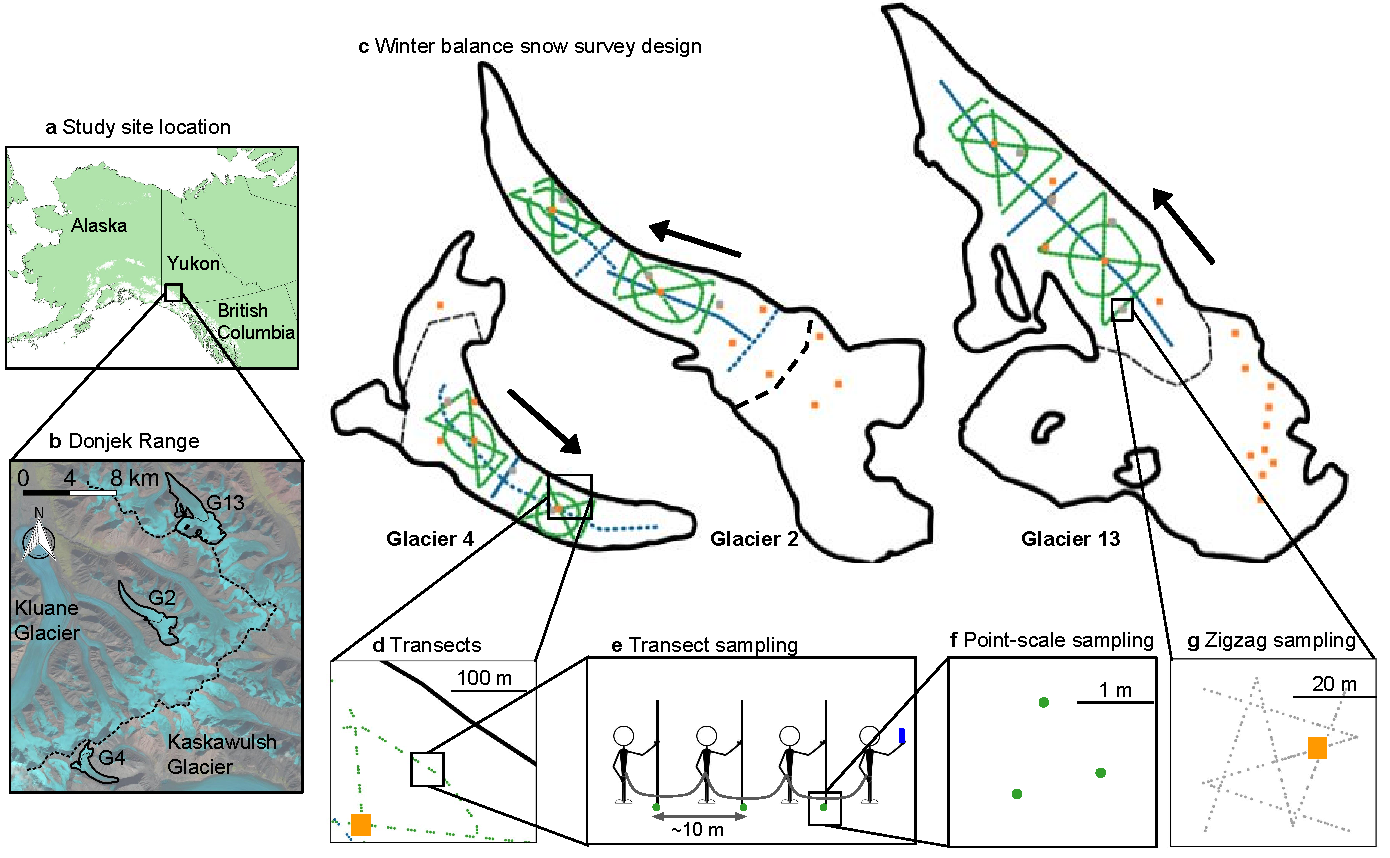
\includegraphics[width =0.9\textwidth]{Sampling.pdf}\\
	\caption{Study area location and sampling design for Glaciers 4, 2 and 13. (a) Study region in the Donjek Range of the St. Elias Mountains of Yukon, Canada. (b) Study glaciers located along a southwest-northeast transect through the Donjek Range. The local topographic divide is shown as a dashed line. Imagery from Landsat8 (5 September 2013, data available from the U.S. Geological Survey). (c) Details of the snow-survey sampling design, with centreline and transverse transects (blue dots), hourglass and circle designs (green dots) and locations of snow density measurements (orange squares). Arrows indicate ice-flow directions. Approximate location of ELA on each glacier is shown as a black dashed line. (d) Close up of linear and curvilinear transects. (e) Configuration of navigator and observers. (f) Point-scale snow-depth sampling. (g) Linear-random snow-depth measurements in `zigzag' design (grey dots) with one density measurement (orange square) per zigzag.}
	\label{fig:Sampling}
\end{figure*}

\section{Study site}

We investigate WB on three unnamed glaciers in the Donjek Range of the St. Elias Mountains (Figure 1). Glacier 4, Glacier 2 and Glacier 13 (labelling adopted from \cite{Crompton2016}) are located along a southwest-northeast transect through the range. These small alpine glaciers have simple geometries and are generally oriented southeast-northwest in valleys with steep walls. See \cite{Pulwicki2017} for a detailed description of sampling design and the process adopted to estimate WB on these glaciers. 


\begin{table*}[]
\centering
\caption{Physical characteristics of the study glaciers and May 2016 winter-balance survey details, including number of snow-depth measurement locations along transects ($n_{\mathrm{T}}$), total length of transects ($d_{\mathrm{T}}$), number of combined snow pit and Federal Sampler density measurement locations ($n_{\rho}$) and number of zigzag surveys ($n_{\mathrm{zz}}$).}
\label{tab:GlacierDetails}
\begin{tabular}{cccccccccccc}
\midrule
\textbf{} & \textbf{Location} & \multicolumn{3}{c}{\textbf{Elevation (m a.s.l)}} & \textbf{Slope ($^{\circ}$)} & \multirow{2}{*}{\textbf{\begin{tabular}[c]{@{}c@{}}Area \\ (km$^2$)\end{tabular}}} & \multirow{2}{*}{\textbf{\begin{tabular}[c]{@{}c@{}}Survey\\ Dates\end{tabular}}} & \multicolumn{4}{c}{\textbf{Survey Details}} \\
 & UTM Zone 7 & \textit{Mean} & \textit{Range} & \textit{ELA} & \textit{Mean} &  &  & $n_{\mathrm{T}}$ & $d_{\mathrm{T}}$ (km) & $n_{\rho}$ & $n_{\mathrm{zz}}$ \\ \midrule
\textbf{Glacier 4} & \begin{tabular}[c]{@{}c@{}}595470 E\\ 6740730 N\end{tabular} & 2344 & 1958--2809 & $\sim$2500 & 12.8 & 3.8 & 4--7 May 2016 & 649 & 13.1 & 10 & 3 \\
\textbf{Glacier 2} & \begin{tabular}[c]{@{}c@{}}601160 E\\ 6753785 N\end{tabular} & 2495 & 1899--3103 & $\sim$2500 & 13.0 & 7.0 & 8--11 May 2016 & 762 & 13.6 & 11 & 3 \\
\textbf{Glacier 13} & \begin{tabular}[c]{@{}c@{}}604602 E\\ 6763400 N\end{tabular} & 2428 & 1923--3067 & $\sim$2380 & 13.4 & 12.6 & 12--15 May 2016 & 941 & 18.1 & 20 & 4
\end{tabular}
\end{table*}

%%%%%%%%%%%%%%%%%%%%%%%%%%%%%%%%%
%	METHODS
%%%%%%%%%%%%%%%%%%%%%%%%%%%%%%%%%


\section{Methods}

Random design too!

We assume a spatial distribution of WB on the three study glaciers, which is equivalent to the distribution presented in \cite{Pulwicki2017}. The assumed WB is estimated using a linear regression fitted to WB data on each glacier, which is obtained from direct measurements of snow depth and density. All estimated values of WB that are calculated using various sampling patterns in this paper are compared against this assumed spatial distribution of WB. By using an assumed distribution as the ``true'' distribution of WB, we are able to calculate spatially-resolved error.  

We investigate various sampling patterns that could be used for a snow survey (Figure 2). Midline (M) and midline with transverse transects (M+T) are the most common survey designs used in WB studies \citep[e.g.][]{Kaser2002,Machguth2006}. The midline survey aims to capture changes in WB with elevation and transverse transects provide observation of lateral variations in WB. Hourglass (H) and inscribed circle (C) allow for sampling in multiple directions and are easy to travel (personal communication from C. Parr, 2016). We use hourglass and circle separately and combined as sampling patterns. All sampling patterns are restricted to the ablation area, where terrain is accessible and direct measurements of snow depth are easy to obtain. For each pattern, a number of evenly-spaced measurements ranging from 45 to 100 total locations is selected. Fewer than 45 measurement locations makes it difficult to fit a linear regression to WB data due to instability in inverting matrices. A maximum of 100 measurements is selected because that is the highest possible number of measurement locations along the shortest pattern (midline on Glacier 4). 

To simulate the process of measuring WB from the assumed distribution, we first obtain WB values at selected measurement locations for each sampling pattern. Then, we add a low or high amount of noise to the WB data. Low noise is defined by a normal distribution that is centred at zero and has a standard deviation equal to the mean standard deviation of WB data from high-density gridcell-scale surveys on each glacier \citep[see][for details]{Pulwicki2017}. High noise is defined in the same way as low noise but the standard deviation of the normal distribution is five times larger. The standard deviation of low noise is $\sim$5\% of the glacier-wide WB, while high noise is $\sim$25\% of the glacier-wide WB. A random number from the high or low noise distribution is chosen for each datum and added to the value of WB. 

A linear regression is then used to interpolate the modified values of WB for each glacier by regressing WB on derived topographic parameters. for each glacier. This linear regression model combines cross correlation and Bayesian model averaging to calculate regression coefficients, as described in \cite{Pulwicki2017}. The resulting regression coefficients are then applied to the topographic parameters associated with each gridcell to obtain distributed WB. RMSE is then calculated by taking the square root of the mean difference between all gridcell from the assumed WB distribution and the WB distribution estimated with the subset pattern.

The process of adding random noise to sampled WB values and fitting a regression to estimate WB is repeated 100 times. Each repetition uses a different set of random noise resulting in a range of WB and RMSE values. A mean WB and RMSE from all runs is then calculated. 


%%%%%%%%%%%%%%%%%%%%%%%%%%%%%%%%%%%%%%%%%%%
%%  RESULTS AND DISCUSSION
%%%%%%%%%%%%%%%%%%%%%%%%%%%%%%%%%%%%%%%%%%%
\section{Results and Discussion}

%FIGURES & TABLES
%Fig 1. Study site and assumed WB distribution
%Fig 2. Sampling patterns
%Fig 3. Computer model results  
%	a) Line plot of WB vs n for all sampling (light coloured and thin) and mean WB (dark coloured and thick) for each glacier
%	b) Same as above but RMSE vs n 
%Fig 4. Map of mean (or max?) RMSE for each G (high/low noise) (best/worst pattern)
%
%Fig ?. Stability of subset sampling -> box plot of RMSE from each pattern (which n?)
%
%Table 1. Assumed WB values and high/low noise std.
%
%
%- which is further to travel, hourglass or midline + transects?
%
%
%Questions?
%- optimal sampling size?
%- best sampling pattern?
%- spread of WB estimates and RMSE with noise
%- grid scale variability (i.e. high/low noise) matters?
%- different for each glacier? captures dominant topographic parameter for each glacier?

%%%%%%%%%%%%%%%%%%%%%%%%%%%%%%%%%%
% CONCLUSION
%%%%%%%%%%%%%%%%%%%%%%%%%%%%%%%%%%
\section{Conclusion}


\section{Acknowledgements}

We thank the Kluane First Nation (KFN), Parks Canada and the Yukon Territorial Government for granting us permission to work in KFN Traditional Territory and Kluane National Park and Reserve. We are grateful for financial support provided by the Natural Sciences and Engineering Research Council of  Canada, Simon Fraser University and the Northern Scientific  Training  Program. We kindly acknowledge Kluane Lake Research Station, Sian Williams, Lance Goodwin and Trans North pilot Dion Parker for facilitating field logistics. We are grateful to Alison Criscitiello and Coline Ariagno for all aspects of field assistance and Sarah Furney for assistance with data entry. Thank you to Etienne Berthier for providing us with the SPIRIT SPOT-5 DEM and for assistance in DEM correction. We are grateful to Derek Bingham and Michael Grosskopf for assistance with the statistics, including simple kriging. Luke Wonneck, Leif Anderson and Jeff Crompton all provided thoughtful and constructive comments on drafts of the manuscript.


%----------------------------------------------------------------------------------------
%	REFERENCE LIST
%----------------------------------------------------------------------------------------
%
%\bibliography{MastersLit}
\bibliography{/home/glaciology1/Documents/MastersDocuments/MastersLit}
%\bibliography{/Users/Alexandra/Documents/SFU/MastersDocuments/MastersLit}
\bibliographystyle{igs}

%----------------------------------------------------------------------------------------

\end{document}
